\chapter{Conclusión}
\section{Conclusiones generales}
El uso de algoritmos de Visión Computarizada para tratamiento de
imágenes es aún algo novedoso y poco extendido. Sin embargo, su
potencial es altísimo. Incluso con unos conocimientos previos
casi inexistentes, en este proyecto ha quedado claro la gran
versatilidad de estas técnicas aplicadas a casos concretos del
mundo real. Aún queda mucho por investigar en este campo de la
informática, y es para nosotros un orgullo haber tenido la 
posibilidad de participar en un trabajo de estas características.\\
Cuando se habla de Visión Computarizada quizá se tienda a pensar,
inocentemente, que es un ámbito específico de la Informática. Sin
embargo va mucho más allá, pues sus funcionalidades son aplicables
a cualquier tipo de imagen, como en este caso lo han sido las 
\emph{tomografías}. Los resultados obtenidos en su tratamiento han
sido más que satisfactorios, tanto para nosotros como para el 
personal médico que ha colaborado en el proyecto, proporcionando
conocimiento técnico del área e imágenes de estudio.

\section{Conclusiones sobre la detección de poros en la papila}
La detección de poros en la papila óptica ha sido un éxito gracias,
en parte, a la biblioteca SimpleCV y sus funcionalidades para 
detectar \emph{blobs}. Se ha logrado un tiempo de procesamiento ínfimo 
comparado con el tiempo empleado por personal médico en marcarlos.
Además, su medición es mucho más precisa que la estimación, hecha
a ojo, que se usaba hasta ahora. \\
A continuación se muestra un ejemplo:

    \begin{figure}[H]
      \caption{Imagen original}
      \centering \setlength\fboxsep{0pt} \setlength\fboxrule{0.5pt}
      \fbox{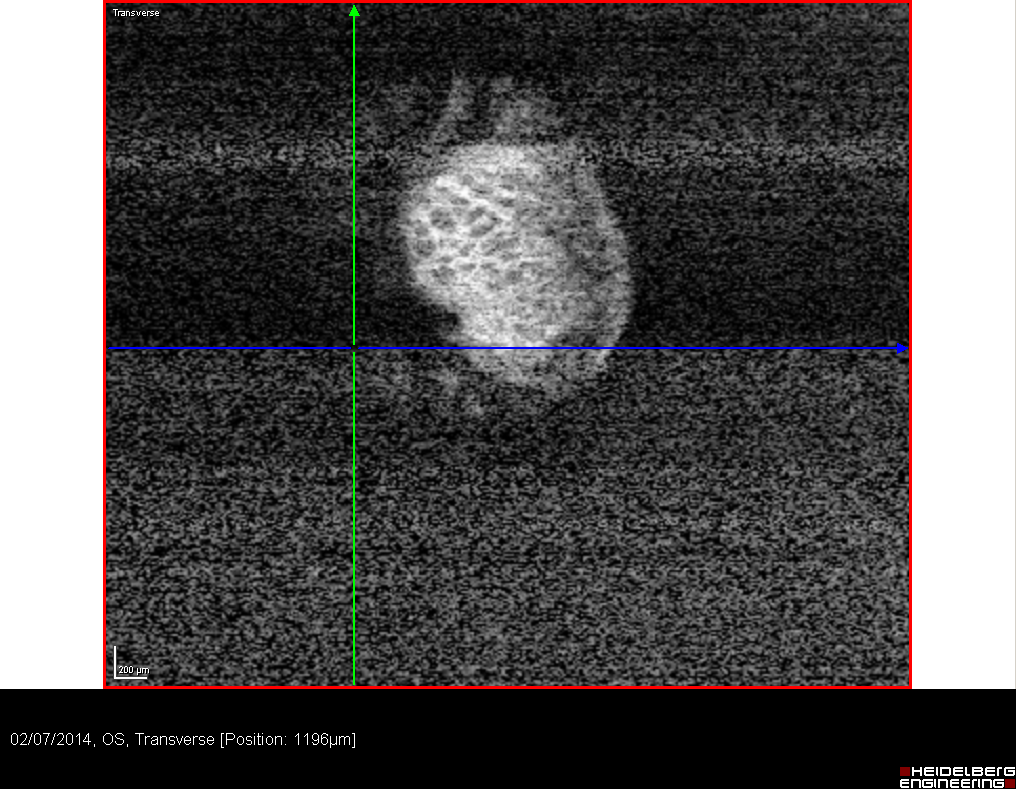
\includegraphics[scale=0.4]{imagenes/conclusiones/PorosOriginal.png}}
    \end{figure}

Con el método que se usaba hasta ahora se obtenía lo siguiente:

    \begin{figure}[H]
      \caption{Imagen marcada por personal médico}
      \centering \setlength\fboxsep{0pt} \setlength\fboxrule{0.5pt}
      \fbox{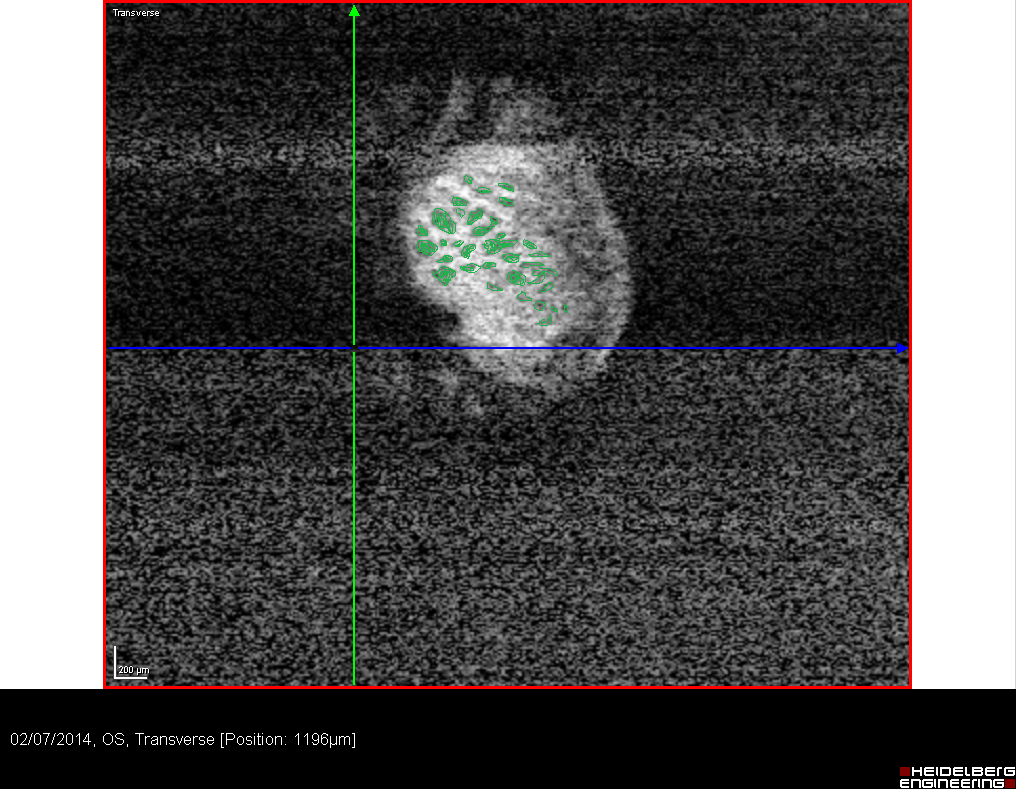
\includegraphics[scale=0.4]{imagenes/conclusiones/PorosMedicos.png}}
    \end{figure}

Nuestros algoritmos detectan más poros como se muestra en las siguientes imágenes. \\
Algoritmo en OpenCV:\@

    \begin{figure}[H]
      \caption{Algoritmo OpenCV}
      \centering \setlength\fboxsep{0pt} \setlength\fboxrule{0.5pt}
      \fbox{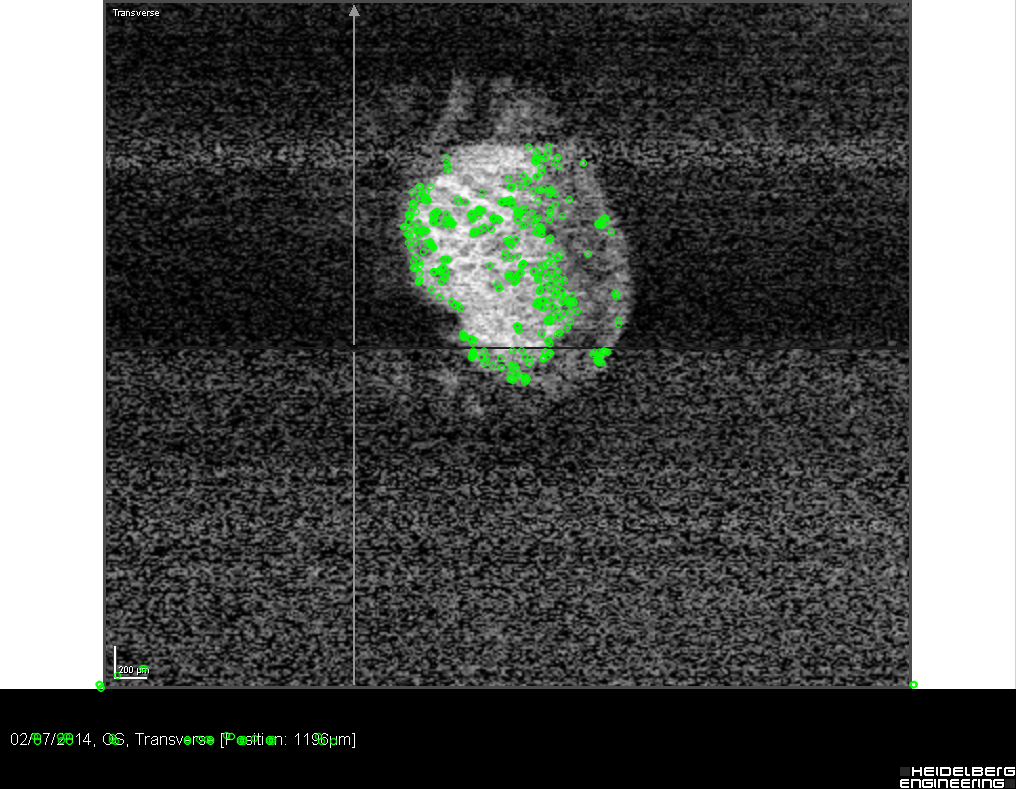
\includegraphics[scale=0.28]{imagenes/conclusiones/PorosOpenCV.png}}
    \end{figure}

Algoritmo usando SimpleCV (en rojo el centro de los poros):

    \begin{figure}[H]
      \caption{Algoritmo SimpleCV}
      \centering \setlength\fboxsep{0pt} \setlength\fboxrule{0.5pt}
      \fbox{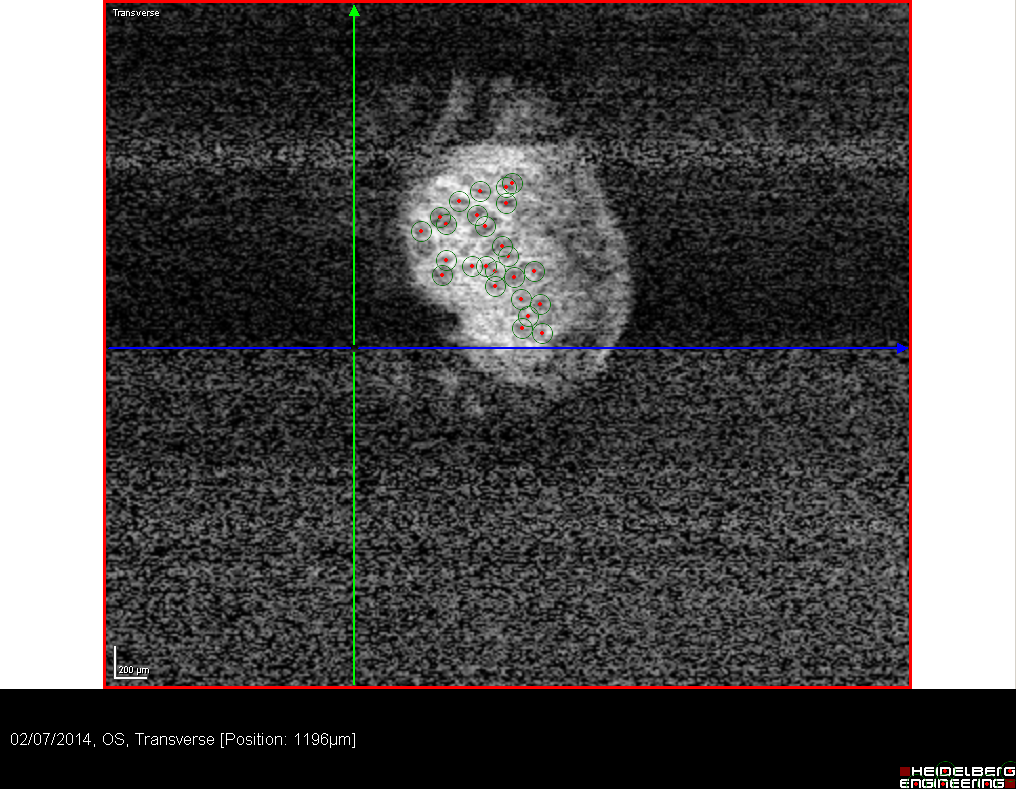
\includegraphics[scale=0.3]{imagenes/conclusiones/PorosSimpleCV.png}}
    \end{figure}

Además de una detección más rápida y fiable, se devuelven los valores exactos del
tamaño de los poros. De esta forma no es necesario estimar la proporción de poros
sobre la superficie de la papila.

\section{Conclusiones sobre la medición del espesor de la coroides}
En cuanto al uso de algoritmos de Visión Computarizada para la 
medición del espesor de la \emph{coroides} los resultados no
podrían ser mejores: se ha alcanzado una precisión de la medición
exacta para la gran mayoría de las imágenes y diferencias 
imperceptibles en los peores casos, cuando el ruido o la calidad
de la imagen complican la detección de los puntos. También se
ha reducido el tiempo de procesamiento, que hasta ahora se hacía
a mano, a menos de un segundo y sin necesidad de intervención
por parte de los oftalmólogos. Esto hace que se eliminen imprecisiones
debido a fallos humanos, como se puede apreciar en el siguiente ejemplo:

    \begin{figure}[H]
      \caption{Medición realizada a mano}
      \centering \setlength\fboxsep{0pt} \setlength\fboxrule{0.5pt}
      \fbox{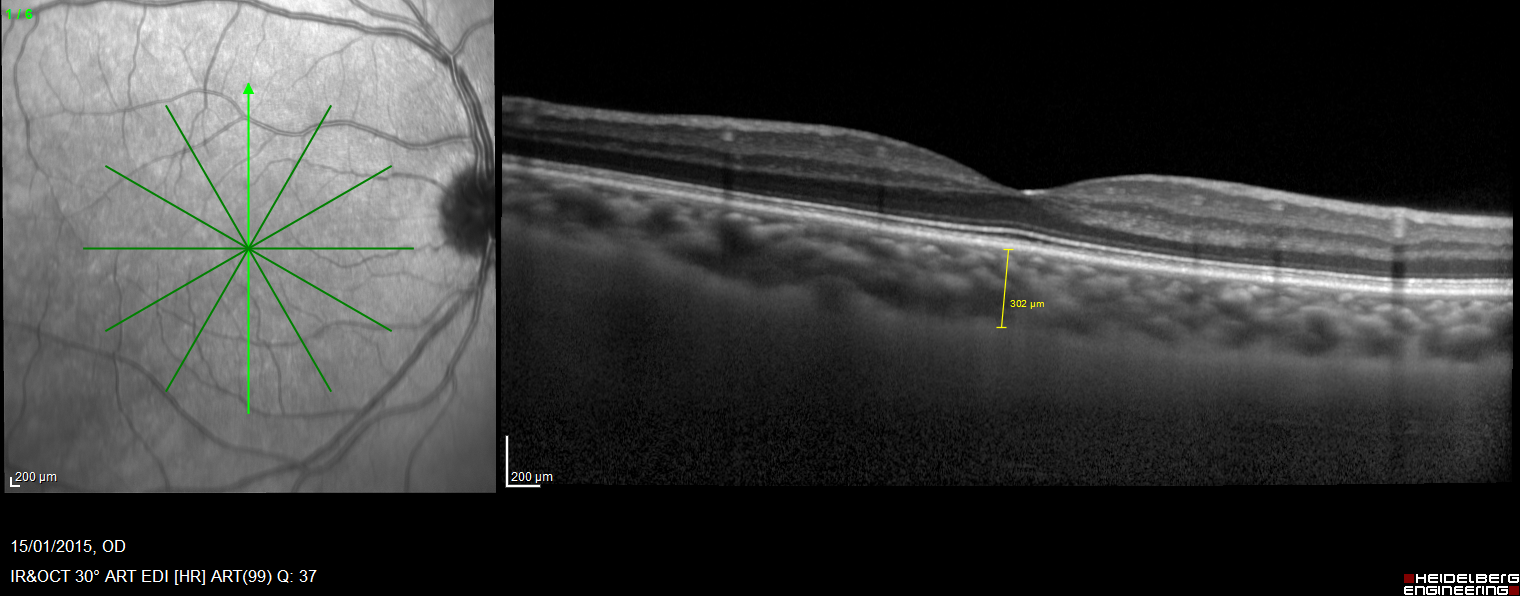
\includegraphics[width=\textwidth]{imagenes/conclusiones/EjemploConclusionMedicos.png}}
    \end{figure}

Si utilizamos nuestro algoritmo y combinamos las imágenes para poder
comparar:

    \begin{figure}[H]
      \caption{Medición realizada con nuestro algoritmo}
      \centering \setlength\fboxsep{0pt} \setlength\fboxrule{0.5pt}
      \fbox{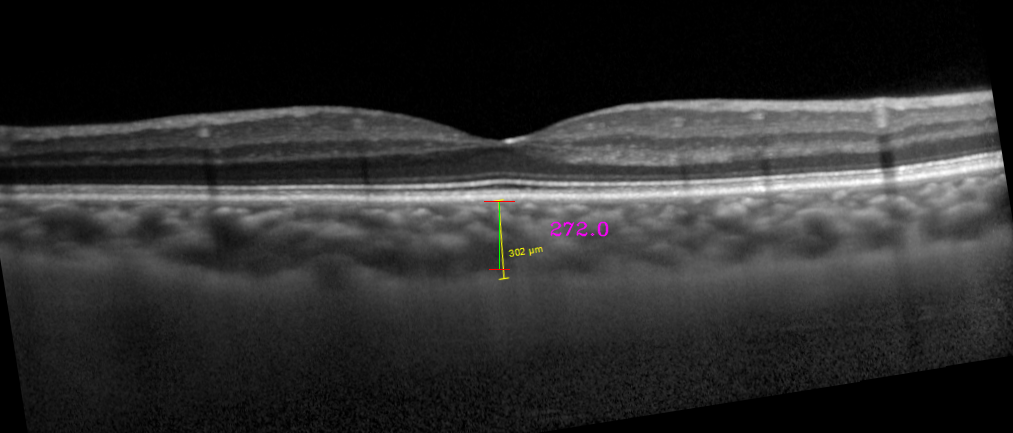
\includegraphics[width=\textwidth]{imagenes/conclusiones/EjemploConclusionCombinada.png}}
    \end{figure}

Se puede apreciar como la recta trazada a mano (en amarillo) se desvía 
hacia la derecha, debido a que al cerebro le cuesta trazar una línea
perpendicular cuando la imagen está girada.\\
También se deja de tener en cuenta el halo generado por el reflejo de la luz
incidente sobre el tejido que puede llevar a fallos en la medición.

